\documentclass{beamer}
\usetheme[progressbar=frametitle,block=fill]{metropolis}           % Use metropolis theme

\usepackage[spanish]{babel}
\usepackage[utf8]{inputenc}
\usepackage{tikz}


\title{Pruebas de Conocimiento Cero y sus Aplicaciones}
\date{\today}
\author{José Luis Cánovas Sánchez\\[3mm]\scriptsize Tutores:\\Antonio José Pallarés Ruiz\\Leandro Marín Muñoz}

\institute{Universidad de Murcia\\Facultad de Matemáticas}
\begin{document}
\maketitle

\begin{frame}
	\frametitle{Outline}
	\tableofcontents
\end{frame}

\section{Problems}

\subsection{Graph Problems}
\begin{frame}{Graph Isomorphism}
	\begin{description}[Question]
		\item[Name] Graph Isomorphism Problem (GI).
		\item[Instance] Given two graphs $G_1 = (V_1, E_1)$ and $G_2 = (V_2, E_2)$ with $\mid V_1 \mid = \mid V_2 \mid = n$.
		\item[Question] Is there a permutation $\tau : V_1 \rightarrow V_2$ such that an edge $(u,v)\in E_1$ if and only if $(\tau (u),\tau (v)) \in E_2$?
	\end{description}



		
\begin{center}
		% Define style for nodes
	\tikzstyle{every node}=[circle, draw, fill=black!50, inner sep=0pt, minimum width=4pt]
	%  Tutte's 8-cage
	\begin{tikzpicture}[thick,scale=0.5]
	% The following path utilizes several useful tricks and features:
	% 1) The foreach statement is put inside a path, so all the edges
	%    will in fact be a the same path.
	% 2) The node construct is used to draw the nodes. Nodes are special
	%    in the way that they are drawn *after* the path is drawn. This
	%    is very useful in this case because the nodes will be drawn on
	%    top of the path and therefore hide all edge joins.
	% 3) Simple arithmetics can be used when specifying coordinates.
	\draw \foreach \x in {0,36,...,324}
	{
		(\x:2) node {}  -- (\x+108:2)
		(\x-10:3) node {} -- (\x+5:4)
		(\x-10:3) -- (\x+36:2)
		(\x-10:3) --(\x+170:3)
		(\x+5:4) node {} -- (\x+41:4)
	};
	\end{tikzpicture}\quad
	\begin{tikzpicture}[thick,scale=0.5]
	\draw \foreach \x in {0,36,...,324}
	{
		(\x:2.5) node {}  -- (\x+108:2.5)
		(\x-10:4) node {} -- (\x+5:1)
		(\x-10:4) -- (\x+36:2.5)
		(\x-10:4) --(\x+170:4)
		(\x+5:1) node {} -- (\x+41:1)
	};
	\end{tikzpicture}
\end{center}
\end{frame}


\begin{frame}{Hamiltonian Cycle \textsuperscript{NPC}}
\begin{description}[Question]
	\item[Name] Hamiltonian Cycle Problem (HC).
	\item[Instance] Given graph $G=(V,E)$.
	\item[Question] Does there exist a Hamiltonian cycle in $G$?
\end{description}

\begin{center}
	\tikzstyle{every node}=[circle, draw, fill=black!50, inner sep=0pt, minimum width=8pt]
\begin{tikzpicture}[thick]
	\draw [line width=0.8mm,purple](120:2) -- (240:2) -- (0:2) -- (0:0) -- cycle;
	\draw (120:2) node {} -- (0:2) node {};
	\draw (0:0) node {} -- (240:2) node {};
\end{tikzpicture}
\end{center}

\end{frame}


\begin{frame}{Graph 3-colorability \textsuperscript{NPC}}

\begin{description}[Question]
	\item[Name] Graph 3-colorability Problem (G3C).
	\item[Instance] Given graph $G=(V,E)$.
	\item[Question] Is there a function	$\phi : V \to \{1,2,3\}$ such that $\phi(u)\neq \phi(v) \quad \forall (u,v)\in E$?
\end{description}

\begin{center}
	\begin{tikzpicture}[style=thick]
	\draw (18:2cm) -- (90:2cm) -- (162:2cm) -- (234:2cm) --
	(306:2cm) -- cycle;
	\draw (18:1cm) -- (162:1cm) -- (306:1cm) -- (90:1cm) --
	(234:1cm) -- cycle;
	\foreach \x in {18,90,162,234,306}{
		\draw (\x:1cm) -- (\x:2cm);
	}
	\draw (18:2cm) circle (5pt)[fill=blue!50];
	\draw (90:2cm) circle (5pt)[fill=green!50];
	\draw (162:2cm) circle (5pt)[fill=red!50];
	\draw (234:2cm) circle (5pt)[fill=green!50];
	\draw (306:2cm) circle (5pt)[fill=red!50];
	
	\draw (18:1cm) circle (5pt)[fill=red!50];%4
	\draw (162:1cm) circle (5pt)[fill=blue!50];%2
	\draw (306:1cm) circle (5pt)[fill=green!50];%5
	\draw (90:1cm) circle (5pt)[fill=red!50];%3
	\draw (234:1cm) circle (5pt)[fill=blue!50];%1
\end{tikzpicture}
\end{center}

\end{frame}


\begin{frame}{Quadratic residue}
	\begin{description}[Question]
		\item[Name] Factorization problem (FACT).
		\item[Instance] Positive integer $N$.
		\item[Question] Are there integers $p,q\geq 2$ such that $N = pq$?
	\end{description}

	\begin{description}[Question]
		\item[Name] Quadratic residue problem (QR).
		\item[Instance] Given a composite integer $N=pq$ and the integer $x$ with Jacobi Symbol $\left( \frac{x}{N} \right) = 1$.
		\item[Question] Is $x$ a quadratic residue in ${\mathbb Z}_N$? $\exists a\in {\mathbb Z}_N : x\equiv a^2 (N)$?
	\end{description}

	\begin{theorem}
		$QR \leq_P FACT$
	\end{theorem}

\end{frame}



\begin{frame}{Discrete Logarithm}

	\begin{description}[Question]
		\item[Name] Discrete Logarithm problem (DL).
		\item[Instance] A cyclic group $G=\left\langle g \right\rangle$ of prime order $q$, an element $y\in G$.
		\item[Question] What is the integer  $s\in \mathbb{Z}_q$ such that $g^s = y$, or $log_g y = s$?
	\end{description}

	\begin{columns}

		\begin{column}{0.5\textwidth}
			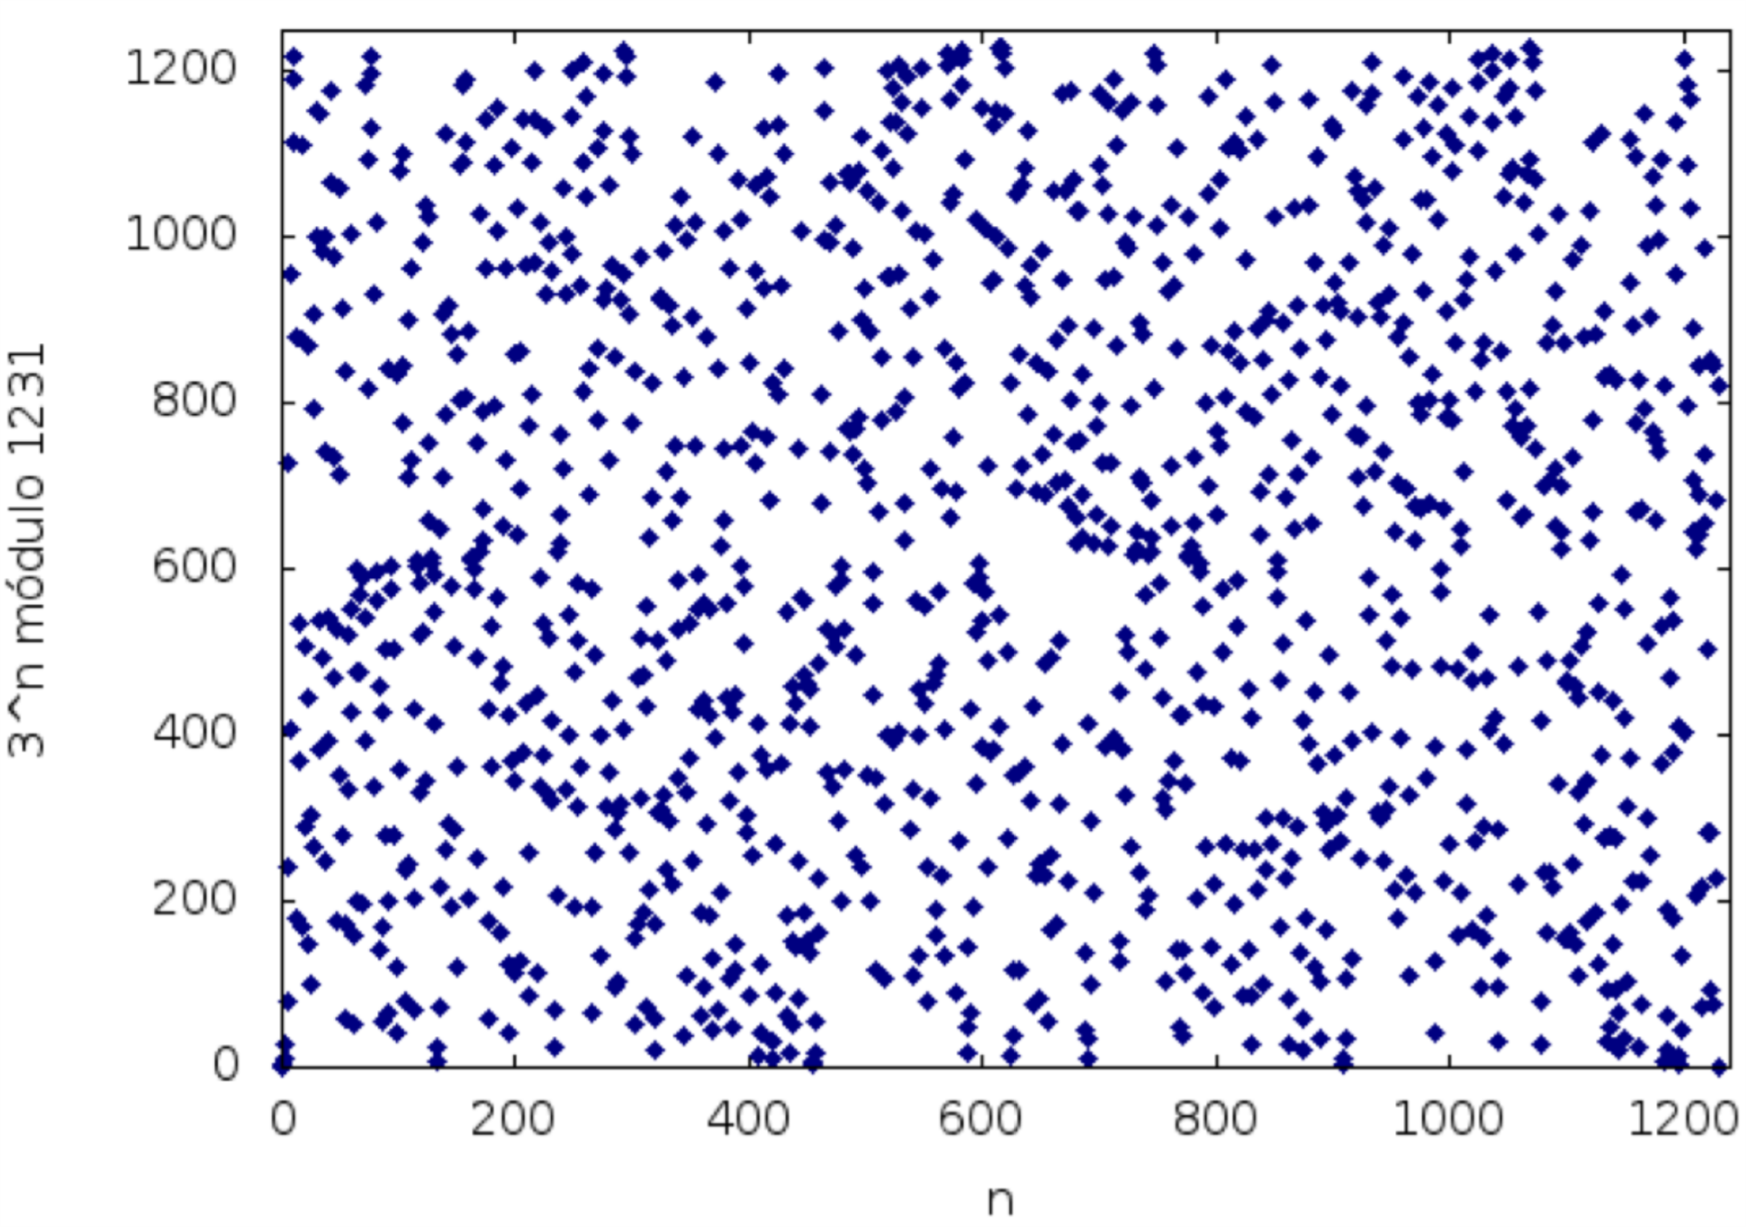
\includegraphics[width=\linewidth]{DL}
		\end{column}
		\begin{column}{0.5\textwidth}
			Discrete Logarithm with $G=\mathbb{Z}_{1231}$, $g=3$.
			
			\small{Adolfo Quirós Gracián. \textit{Grupos y criptografía: de Julio César a las curvas elípticas.}}
		\end{column}
	
	\end{columns}


\end{frame}






\section{Pruebas Interactivas}



\end{document}